
\chapter{Concept Model}
\label{chap:lu.uni.lassy.excalibur.MyCrash.G02-CM}


\section{PrimaryTypes-Classes}
\subsection{Local view 01}
\label{sec:lu.uni.lassy.excalibur.MyCrash.G02-CM-view-local-PrimaryTypes-Classes-01}
Figure \ref{fig:lu.uni.lassy.excalibur.MyCrash.G02-CM-view-local-PrimaryTypes-Classes-01} presents the relations between all the classes.



\begin{figure}[htbp] 
\label{fig:lu.uni.lassy.excalibur.MyCrash.G02-CM}
\begin{center}
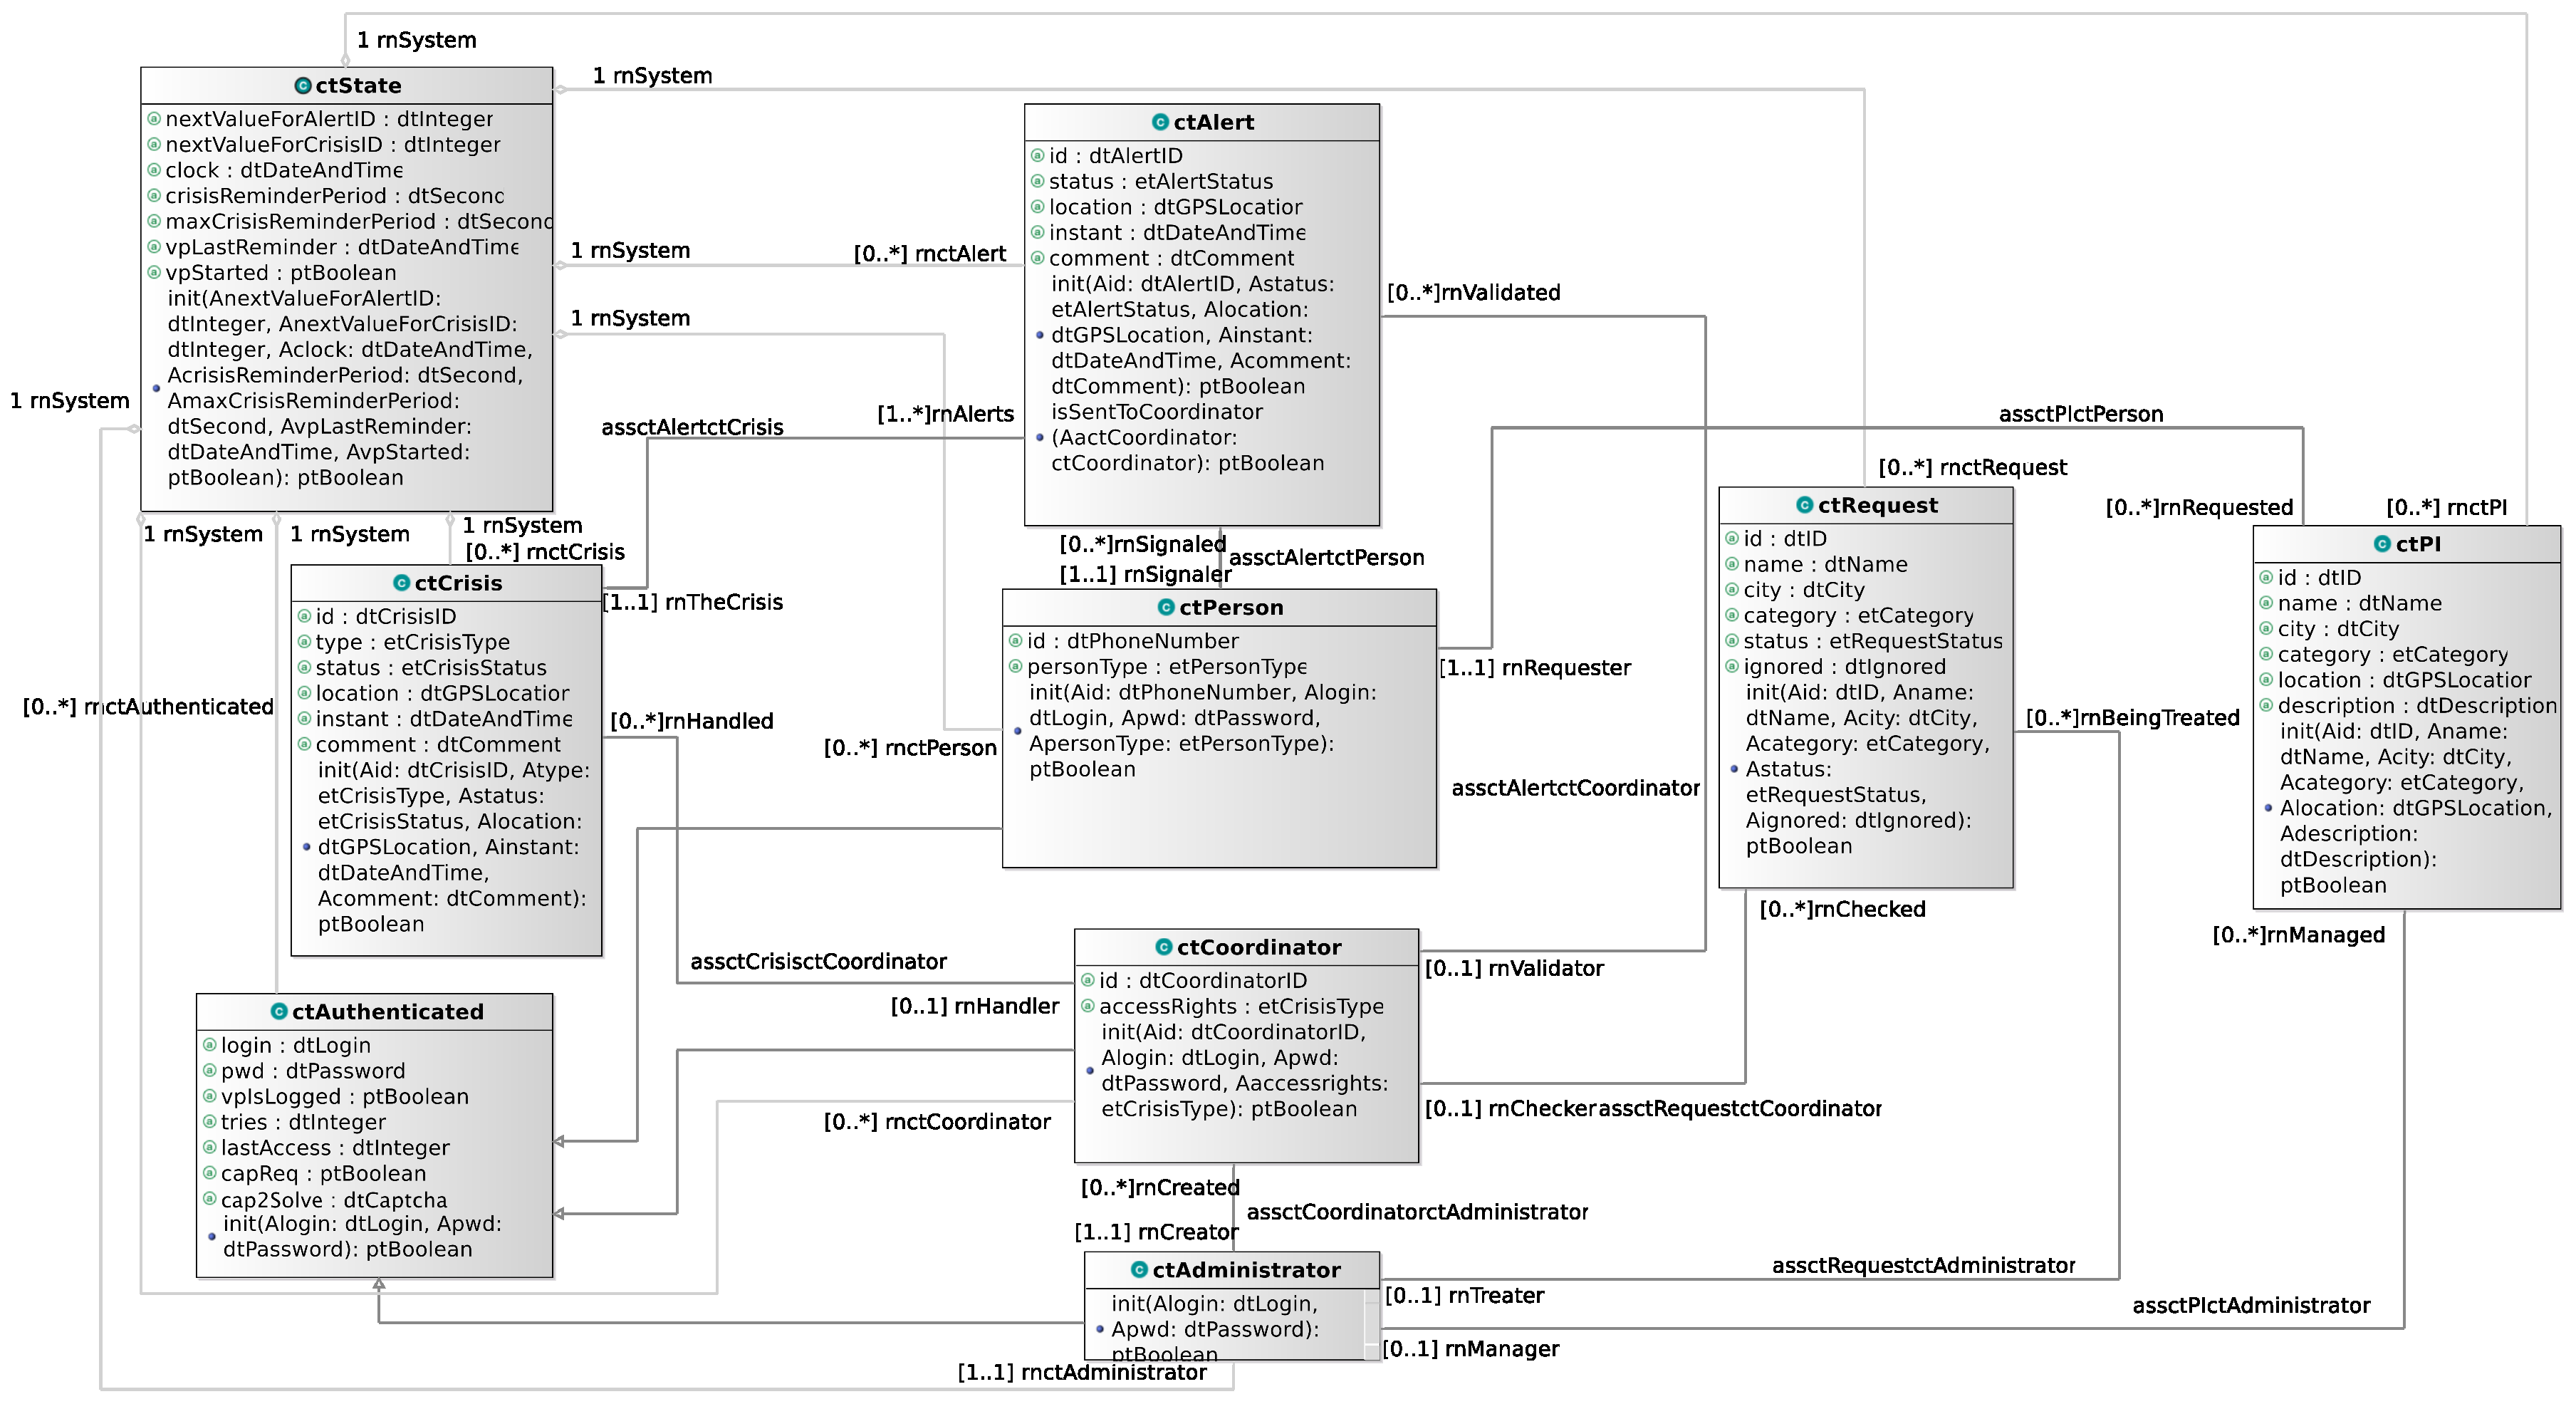
\includegraphics[
angle=90
,height=1.0\textheight
]{./images-report-gen/concept-model/local/PrimaryTypes-Classes/01/PrimaryTypes-CLV-01.eps}
\end{center}
\caption[Concept Model - PrimaryTypes-Classes local view 01 - PrimaryTypes Classes local view 01]{Concept Model - PrimaryTypes-Classes local view 01. PrimaryTypes Classes local view 01.}
\label{fig:lu.uni.lassy.excalibur.MyCrash.G02-CM-view-local-PrimaryTypes-Classes-01}
\end{figure}
\vspace{0.5cm} 


\subsection{Global view 05}
\label{sec:lu.uni.lassy.excalibur.MyCrash.G02-CM-view-global-PrimaryTypes-Classes-05}
Figure \ref{fig:lu.uni.lassy.excalibur.MyCrash.G02-CM-view-global-PrimaryTypes-Classes-05} Represents class-actor relation for the PI variant



\begin{figure}[htbp] 
\label{fig:lu.uni.lassy.excalibur.MyCrash.G02-CM}
\begin{center}
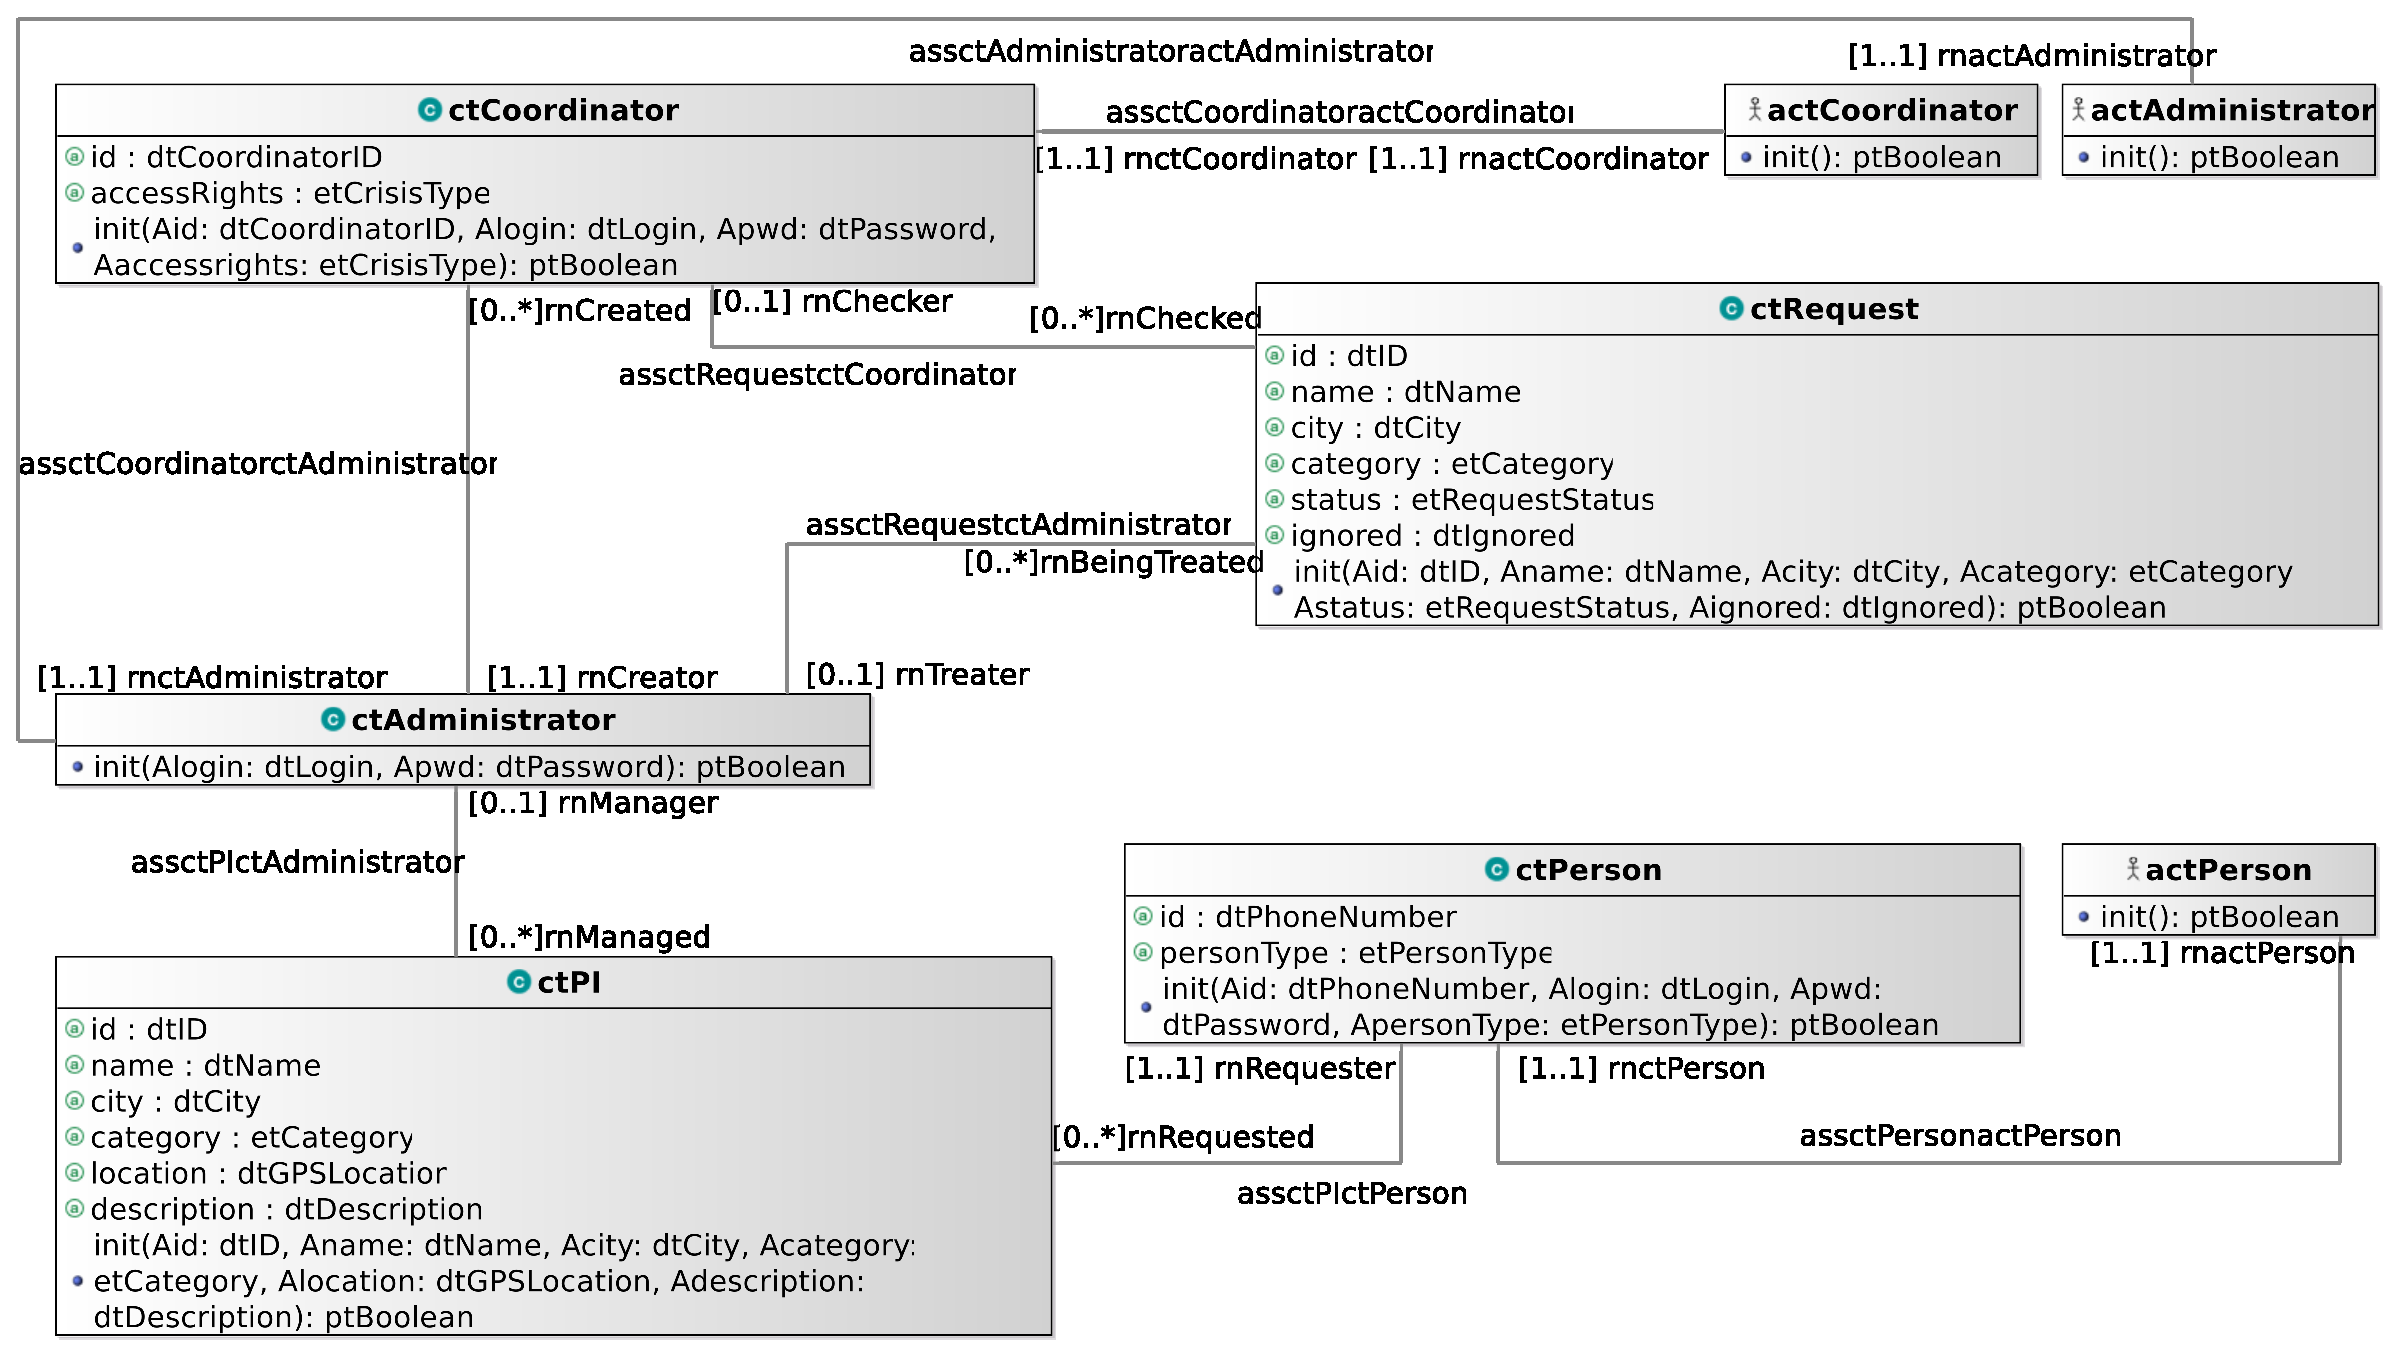
\includegraphics[
angle=0
]{./images-report-gen/concept-model/global/PrimaryTypes-Classes/05/PIvariant-CGV-01.eps}
\end{center}
\caption[Concept Model - PrimaryTypes-Classes global view 05 - PIvariant-CGV-01 concept global view]{Concept Model - PrimaryTypes-Classes global view 05. PIvariant-CGV-01 concept global view 01.}
\label{fig:lu.uni.lassy.excalibur.MyCrash.G02-CM-view-global-PrimaryTypes-Classes-05}
\end{figure}
\vspace{0.5cm} 

\subsection{Global view 06}
\label{sec:lu.uni.lassy.excalibur.MyCrash.G02-CM-view-global-PrimaryTypes-Classes-06}
Figure \ref{fig:lu.uni.lassy.excalibur.MyCrash.G02-CM-view-global-PrimaryTypes-Classes-06} Represents class and actor relation for Access Rights variant.



\begin{figure}[htbp] 
\label{fig:lu.uni.lassy.excalibur.MyCrash.G02-CM}
\begin{center}
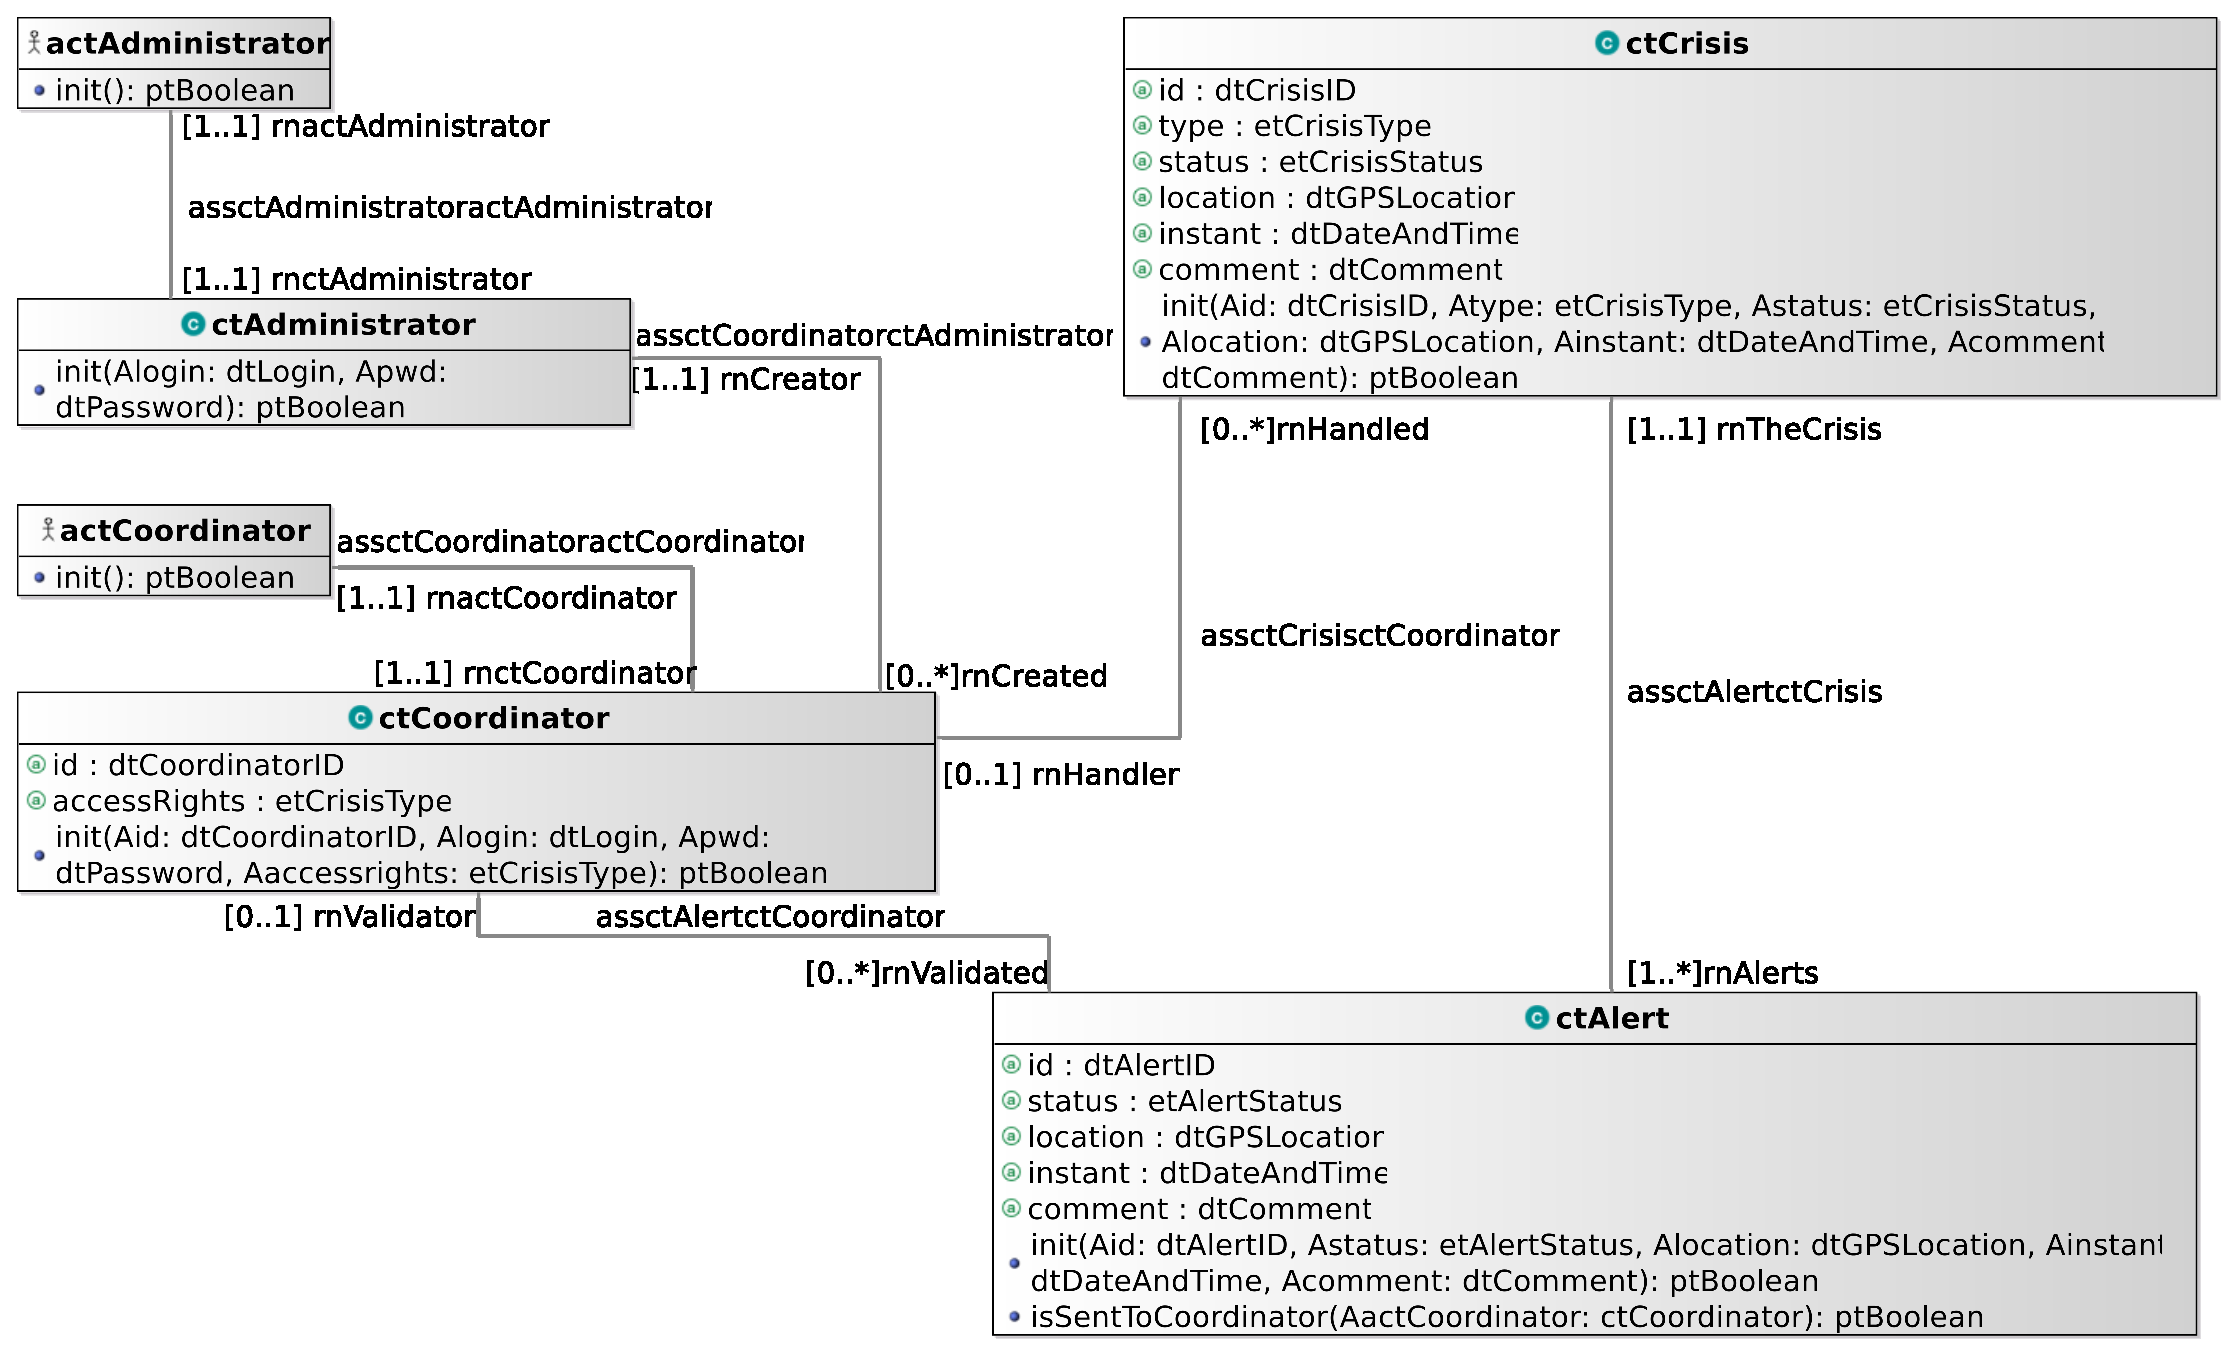
\includegraphics[
angle=0
]{./images-report-gen/concept-model/global/PrimaryTypes-Classes/06/ARvariant-CGV-01.eps}
\end{center}
\caption[Concept Model - PrimaryTypes-Classes global view 06 - ARvariant-CGV-01 concept global view]{Concept Model - PrimaryTypes-Classes global view 06. ARvariant-CGV-01 concept global view 01.}
\label{fig:lu.uni.lassy.excalibur.MyCrash.G02-CM-view-global-PrimaryTypes-Classes-06}
\end{figure}
\vspace{0.5cm} 











\section{Concept Model Types Descriptions}
This section provides the textual descriptions of all the types defined in the concept model and that can be part of the graphical views provided.

\subsection{Primary types - Class types descriptions}




The table below is providing comments on the graphical views given for the class types of the primary types. Type logical operations are precisely specified in the operation model.

\begin{datadictionary}
\addheading{Classes}

\adddoublerow{ctAdministrator}{used to caracterize internally the entity that is responsible of administrating the iCrash system.}
\addsingletwocolumnrow{extends}{lu.uni.lassy.excalibur.MyCrash.G02.concepts.primarytypes.classes.ctAuthenticated}
\adddoubletwocolumnrow{operation}{\msrcode{init(Alogin:dtLogin, Apwd:dtPassword):ptBoolean}}{used to initialize the current object as a new instance of the ctAdministrator type.}
\adddoublerow{ctAlert}{Used to model crisis alerts sent by any human having communication capability using communication
companies belonging to the systems environment}
\adddoubletwocolumnrow{attribute}{\msrcode{comment: dtComment}}{a textual description providing unstructured information on the alert.}
\adddoubletwocolumnrow{attribute}{\msrcode{id: dtAlertID}}{the alert unique identification information.}
\adddoubletwocolumnrow{attribute}{\msrcode{instant: dtDateAndTime}}{the date and time at which the alert notification has been sent.}
\adddoubletwocolumnrow{attribute}{\msrcode{location: dtGPSLocation}}{the position of the alert provided by the space-based satellite navigation system used
by the human using the communication company to inform the iCrash system of a
crisis.}
\adddoubletwocolumnrow{attribute}{\msrcode{status: etAlertStatus}}{the alert validation status}
\adddoubletwocolumnrow{operation}{\msrcode{init(Aid:dtAlertID, Astatus:etAlertStatus, Alocation:dtGPSLocation, Ainstant:dtDateAndTime, Acomment:dtComment):ptBoolean}}{used to initialize the current object as a new instance of the ctAlert type.}
\adddoubletwocolumnrow{operation}{\msrcode{isSentToCoordinator(AactCoordinator:ctCoordinator):ptBoolean}}{used to provide a given coordinator with current alert information.}
\adddoublerow{ctAuthenticated}{used to model systems representation about actors that need to authenticate to access some specific
functionalities.}
\adddoubletwocolumnrow{attribute}{\msrcode{capReq: ptBoolean}}{used to determine if the actor needs to solve a captcha.}
\adddoubletwocolumnrow{attribute}{\msrcode{lastAccess: dtInteger}}{used to determine the last time the actor tried to login.}
\adddoubletwocolumnrow{attribute}{\msrcode{login: dtLogin}}{an identifier for authentication.}
\adddoubletwocolumnrow{attribute}{\msrcode{pwd: dtPassword}}{a key for authentication.}
\adddoubletwocolumnrow{attribute}{\msrcode{tries: dtInteger}}{used to determine how many tries the actor tried to login.}
\adddoubletwocolumnrow{attribute}{\msrcode{vpIsLogged: ptBoolean}}{used to determine the access status.}
\adddoubletwocolumnrow{operation}{\msrcode{init(Alogin:dtLogin, Apwd:dtPassword):ptBoolean}}{used to initialize the current object as a new instance of the ctAuthenticated type.}
\adddoublerow{ctCoordinator}{used to model systems representation about the actors that have the responsibility to handle alerts
and crisis.}
\addsingletwocolumnrow{extends}{lu.uni.lassy.excalibur.MyCrash.G02.concepts.primarytypes.classes.ctAuthenticated}
\adddoubletwocolumnrow{attribute}{\msrcode{id: dtCoordinatorID}}{a unique identification information.}
\adddoubletwocolumnrow{operation}{\msrcode{init(Aid:dtCoordinatorID, Alogin:dtLogin, Apwd:dtPassword, Aaccessrights:etCrisisType):ptBoolean}}{used to initialize the current object as a new instance of the ctCoordinator type.}
\adddoublerow{ctCrisis}{Used to model crisis that are infered from the reception of at least one alert message. Crisis are entities
that are handled by the iCrash system.}
\adddoubletwocolumnrow{attribute}{\msrcode{comment: dtComment}}{a textual description providing unstructured information on the crisis handling.}
\adddoubletwocolumnrow{attribute}{\msrcode{id: dtCrisisID}}{the crisis unique identification information.}
\adddoubletwocolumnrow{attribute}{\msrcode{instant: dtDateAndTime}}{the date and time at which the first related alert notification has been sent.}
\adddoubletwocolumnrow{attribute}{\msrcode{location: dtGPSLocation}}{the position of the crisis equal by the one of the first alert received and associated to
the crisis.}
\adddoubletwocolumnrow{attribute}{\msrcode{status: etCrisisStatus}}{the crisis handling status.}
\adddoubletwocolumnrow{attribute}{\msrcode{type: etCrisisType}}{an indication of the gravity of the crisis.}
\adddoubletwocolumnrow{operation}{\msrcode{init(Aid:dtCrisisID, Atype:etCrisisType, Astatus:etCrisisStatus, Alocation:dtGPSLocation, Ainstant:dtDateAndTime, Acomment:dtComment):ptBoolean}}{used to initialize the current object as a new instance of the ctAlert type.}
\adddoublerow{ctPerson}{Used to model systems representation about the indirect actors that has alerted 
of potential crisis, but also perform requests for new potential points of interest.}
\addsingletwocolumnrow{extends}{lu.uni.lassy.excalibur.MyCrash.G02.concepts.primarytypes.classes.ctAuthenticated}
\adddoubletwocolumnrow{attribute}{\msrcode{id: dtPhoneNumber}}{the persons unique identification information of type dtPhoneNumber.}
\adddoubletwocolumnrow{attribute}{\msrcode{personType: etPersonType}}{the person type.}
\adddoubletwocolumnrow{operation}{\msrcode{init(Aid:dtPhoneNumber, Alogin:dtLogin, Apwd:dtPassword, ApersonType:etPersonType):ptBoolean}}{used to initialise the current object as a new instance of the ctPerson type.}
\adddoublerow{ctPI}{Used to model points of interest that are introduced from the reception of at 
least one request. PIs are handled by the actor Administrator.}
\adddoubletwocolumnrow{attribute}{\msrcode{category: etCategory}}{classifies the PI in a sort of groups.}
\adddoubletwocolumnrow{attribute}{\msrcode{city: dtCity}}{represents the location at the specific point of interest.}
\adddoubletwocolumnrow{attribute}{\msrcode{description: dtDescription}}{a textual description providing information of the point of interest.}
\adddoubletwocolumnrow{attribute}{\msrcode{id: dtID}}{the PIs unique identification information.}
\adddoubletwocolumnrow{attribute}{\msrcode{location: dtGPSLocation}}{represents the location of the PI as GPS coordinates.}
\adddoubletwocolumnrow{attribute}{\msrcode{name: dtName}}{represents the name of a point of interest.}
\adddoubletwocolumnrow{operation}{\msrcode{init(Aid:dtID, Aname:dtName, Acity:dtCity, Acategory:etCategory, Alocation:dtGPSLocation, Adescription:dtDescription):ptBoolean}}{used to initialise the current object as a new instance of the ctPI type.}
\adddoublerow{ctRequest}{Used to model requests that are introduced from the actor Person as a new potential 
point of interest.}
\adddoubletwocolumnrow{attribute}{\msrcode{category: etCategory}}{classifies the new potential PI in a sort of groups.}
\adddoubletwocolumnrow{attribute}{\msrcode{city: dtCity}}{represents the location at the new potential point of interest.}
\adddoubletwocolumnrow{attribute}{\msrcode{id: dtID}}{the request's unique identification information.}
\adddoubletwocolumnrow{attribute}{\msrcode{ignored: dtIgnored}}{represents the fact that the new to add point of interest already exists or not. 
Shall be ignored if yes.}
\adddoubletwocolumnrow{attribute}{\msrcode{name: dtName}}{represents the potential name of the new point of interest.}
\adddoubletwocolumnrow{attribute}{\msrcode{status: etRequestStatus}}{the request handling status.}
\adddoubletwocolumnrow{operation}{\msrcode{init(Aid:dtID, Aname:dtName, Acity:dtCity, Acategory:etCategory, Astatus:etRequestStatus, Aignored:dtIgnored):ptBoolean}}{used to initialise the current object as a new instance of the ctRequest type.}
\adddoublerow{ctState}{used to model the system. Each system specified using Messir must include a ctState class for
which there is only one instance at any state of the abstract machine after creation.}
\adddoubletwocolumnrow{attribute}{\msrcode{clock: dtDateAndTime}}{used to represent the system local time.}
\adddoubletwocolumnrow{attribute}{\msrcode{crisisReminderPeriod: dtSecond}}{used to define the delay between two reminders after which a reminder must be sent
to the administrator and to the known coordinators to encourage them to handle the
crisis.}
\adddoubletwocolumnrow{attribute}{\msrcode{maxCrisisReminderPeriod: dtSecond}}{used to define the maximum delay after which the crisis is ramdomly allocated to a
coordinator if any or an alert message is sent to the administrator in order to encourage
him to add coordinators.}
\adddoubletwocolumnrow{attribute}{\msrcode{nextValueForAlertID: dtInteger}}{nextValueForAlertID: dtInteger: used to associate each alert declared with
a unique idenitification value.}
\adddoubletwocolumnrow{attribute}{\msrcode{nextValueForCrisisID: dtInteger}}{used to associate each crisis declared with a unique idenitification value.}
\adddoubletwocolumnrow{attribute}{\msrcode{vpLastReminder: dtDateAndTime}}{date and time of the last reminder.}
\adddoubletwocolumnrow{attribute}{\msrcode{vpStarted: ptBoolean}}{used to avoid reacting to an actor message if the system is not started (i.e.
oeCreateSystemAndEnvironment not executed).}
\adddoubletwocolumnrow{operation}{\msrcode{init(AnextValueForAlertID:dtInteger, AnextValueForCrisisID:dtInteger, Aclock:dtDateAndTime, AcrisisReminderPeriod:dtSecond, AmaxCrisisReminderPeriod:dtSecond, AvpLastReminder:dtDateAndTime, AvpStarted:ptBoolean):ptBoolean}}{used to initialize the current object as a new instance of the ctState type.}
\end{datadictionary}

\subsection{Primary types - Datatypes types descriptions}





The table below is providing comments on the graphical views given for the datatype types of the primary types.


\begin{datadictionary}
\addheading{Datatypes}

\adddoublerow{dtAdministratorID}{A string used to identify the administrator.}
\addsingletwocolumnrow{extends}{dtString}
\adddoubletwocolumnrow{operation}{\msrcode{is():ptBoolean}}{used to determine which strings are considered as valid administrator identifiers.}
\adddoublerow{dtAlertID}{A string used to identify alerts.}
\addsingletwocolumnrow{extends}{dtString}
\adddoubletwocolumnrow{operation}{\msrcode{is():ptBoolean}}{used to determine which strings are considered as valid alert identifiers.}
\adddoublerow{dtCaptcha}{A string used to store the Captcha information after the iCrash user failed to log in 
three times.}
\addsingletwocolumnrow{extends}{dtString}
\adddoubletwocolumnrow{operation}{\msrcode{is():ptBoolean}}{used to determine which strings are considered as valid dtCaptcha.}
\adddoublerow{dtCity}{A string used to store the name of the city in which the point of interest is situated.}
\addsingletwocolumnrow{extends}{dtString}
\adddoubletwocolumnrow{operation}{\msrcode{is():ptBoolean}}{used to determine which strings are considered as valid dtCity.}
\adddoublerow{dtComment}{A datatype made of a string value used to receive, store and send textual information 
about crisis and alerts.}
\addsingletwocolumnrow{extends}{dtString}
\adddoubletwocolumnrow{operation}{\msrcode{is():ptBoolean}}{used to determine which strings are considered as valid comments.}
\adddoublerow{dtCoordinatorID}{A string used to identify coordinators.}
\addsingletwocolumnrow{extends}{dtString}
\adddoubletwocolumnrow{operation}{\msrcode{is():ptBoolean}}{used to determine which strings are considered as valid coordinators identifiers.}
\adddoublerow{dtCrisisID}{A string used to identify crisis.}
\addsingletwocolumnrow{extends}{dtString}
\adddoubletwocolumnrow{operation}{\msrcode{is():ptBoolean}}{used to determine which strings are considered as valid crisis identifiers.}
\adddoublerow{dtDescription}{A datatype made of a string value used to receive, store and send textual information about 
a point of interest.}
\addsingletwocolumnrow{extends}{dtString}
\adddoubletwocolumnrow{operation}{\msrcode{is():ptBoolean}}{used to determine which strings are considered as valid descriptions.}
\adddoublerow{dtGPSLocation}{Used to define coordinates of geographical positions on earth. It is defined a couple made of a latitude
and a longitude.}
\addsingletwocolumnrow{extends}{dtString}
\adddoubletwocolumnrow{attribute}{\msrcode{latitude: dtLatitude}}{for the latitude part of the coordinate.}
\adddoubletwocolumnrow{attribute}{\msrcode{longitude: dtLongitude}}{for the longitude part of the coordinate.}
\adddoubletwocolumnrow{operation}{\msrcode{is():ptBoolean}}{used to determine which couples are considered as valid dtGPSLocation values.}
\adddoublerow{dtID}{A string used to identify points of interest and requests.}
\addsingletwocolumnrow{extends}{dtString}
\adddoubletwocolumnrow{operation}{\msrcode{is():ptBoolean}}{used to determine which strings are considered as valid points of interest and request identifiers.}
\adddoublerow{dtIgnored}{A boolean used to store the value considering if the request should be ignored or not.}
\adddoubletwocolumnrow{operation}{\msrcode{is():ptBoolean}}{used to determine which boolean values are considered as valid dtIgnored.}
\adddoublerow{dtLatitude}{Used to define a latitude value of a geographical positions on earth.}
\addsingletwocolumnrow{extends}{dtReal}
\adddoubletwocolumnrow{operation}{\msrcode{is():ptBoolean}}{used to determine which strings are considered as valid dtLatitude.}
\adddoublerow{dtLogin}{A login string used to authentify an iCrash user.}
\addsingletwocolumnrow{extends}{dtString}
\adddoubletwocolumnrow{operation}{\msrcode{is():ptBoolean}}{used to determine which strings are considered as valid dtLogin.}
\adddoublerow{dtLongitude}{Used to define a longitude value of a geographical positions on earth.}
\addsingletwocolumnrow{extends}{dtReal}
\adddoubletwocolumnrow{operation}{\msrcode{is():ptBoolean}}{used to determine which strings are considered as valid dtLongitude.}
\adddoublerow{dtMessage}{A string used to store the information that will be sent as input event to the actors.}
\addsingletwocolumnrow{extends}{dtString}
\adddoubletwocolumnrow{operation}{\msrcode{is():ptBoolean}}{used to determine which strings are considered as valid dtMessage.}
\adddoublerow{dtName}{A string used to store the names of the points of interest.}
\addsingletwocolumnrow{extends}{dtString}
\adddoubletwocolumnrow{operation}{\msrcode{is():ptBoolean}}{used to determine which strings are considered as valid names.}
\adddoublerow{dtPassword}{A password string used to authentify an iCrash user.}
\addsingletwocolumnrow{extends}{dtString}
\adddoubletwocolumnrow{operation}{\msrcode{is():ptBoolean}}{used to determine which strings are considered as valid dtPassword.}
\adddoublerow{dtPhoneNumber}{A string used to store the phone number from the person declaring the crisis or the alert.}
\addsingletwocolumnrow{extends}{dtString}
\adddoubletwocolumnrow{operation}{\msrcode{is():ptBoolean}}{used to determine which strings are considered as valid dtPhoneNumber.}
\end{datadictionary}


\begin{datadictionary}
\addheading{Enumerations}

\adddoublerow{etAlertStatus}{This type is used to indicate the different validation status of an alert.}
\adddoubletwocolumnrow{operation}{\msrcode{is():ptBoolean}}{used to determine which literal belongs to the enumeration.}
\adddoublerow{etCategory}{This type is used to indicate the different categories of a point of interest.}
\adddoubletwocolumnrow{operation}{\msrcode{is():ptBoolean}}{used to determine which literal belongs to the enumeration.}
\adddoublerow{etCrisisStatus}{This type is used to indicate the different handling status of a crisis.}
\adddoubletwocolumnrow{operation}{\msrcode{is():ptBoolean}}{used to determine which literal belongs to the enumeration.}
\adddoublerow{etCrisisType}{This type is used to indicate the different types of a crisis.}
\adddoubletwocolumnrow{operation}{\msrcode{is():ptBoolean}}{used to determine which literal belongs to the enumeration.}
\adddoublerow{etPersonType}{This type is used to indicate the type of person that informs about a car crash crisis.}
\adddoubletwocolumnrow{operation}{\msrcode{is():ptBoolean}}{used to determine which literal belongs to the enumeration.}
\adddoublerow{etRequestStatus}{This type is used to indicate the different status of the request made for a point of interest.}
\adddoubletwocolumnrow{operation}{\msrcode{is():ptBoolean}}{used to determine which literal belongs to the enumeration.}
\end{datadictionary}






\subsection{Primary types - Association types descriptions}




The table below is providing comments on the association types of the primary types.

\begin{associationtypes}
\addheading{Associations}
\adddoublerow{assctAdministratoractAdministrator}{frequent messages must be sent to coordinator especially in relation to coordinators they manage.}
\adddoublerow{assctAlertctCoordinator}{alerts need to be sent to coordinator in order to be validated or invalidated}
\adddoublerow{assctAlertctCrisis}{a crisis is related to one or more alerts as the alerts judged to concern all the same crisis due to their
location. An alert alerts exactly one crisis.}
\adddoublerow{assctAlertctPerson}{alerts are notified by person through the communication company. We need to keep an internal
representation of those person to allow for communication of alert handling.}
\adddoublerow{assctAuthenticatedactAuthenticated}{mainly used to determine if the login request of an authenticated actor can be granted based on the
given credentials and the registered ones.}
\adddoublerow{assctCoordinatoractCoordinator}{frequent messages must be sent to coordinator especially in relation to crisis they handle.}
\adddoublerow{assctCoordinatorctAdministrator}{one administrator manages more coordinators}
\adddoublerow{assctCrisisctCoordinator}{at any point in time we need to know if a coordinator is handling existing crisis or not.}
\adddoublerow{assctPersonactComCompany}{in order to communicate with person who informed about potential crisis, we need to record the
communication company to use to send them messages.}
\adddoublerow{assctPersonactPerson}{messages must be sent to person}
\adddoublerow{assctPIctAdministrator}{one administrator is charge of handling various point of interest}
\adddoublerow{assctPIctPerson}{several people can request several points of interests}
\adddoublerow{assctRequestctAdministrator}{one administrator is charge of handling various point of interest requests}
\adddoublerow{assctRequestctCoordinator}{several coordinators are charge of monitoring various point of interest requests}
\end{associationtypes}

\input{doc-gen/concept-model/comments-tables/primaryTypesAggregations-comments-table.tex}
\input{doc-gen/concept-model/comments-tables/primaryTypesCompositions-comments-table.tex}
\input{doc-gen/concept-model/comments-tables/secondaryTypesClasses-comments-table.tex}
\input{doc-gen/concept-model/comments-tables/secondaryTypesDatatypes-comments-table.tex}
\input{doc-gen/concept-model/comments-tables/secondaryTypesAssociations-comments-table.tex}
\input{doc-gen/concept-model/comments-tables/secondaryTypesAggregations-comments-table.tex}
\input{doc-gen/concept-model/comments-tables/secondaryTypesCompositions-comments-table.tex}

